\documentclass[letterpaper,12pt]{article}
\usepackage[utf8]{inputenc}
\usepackage{graphicx}
\title{\huge{\emph{Vivir lejos no es bonito}}}
\author{Ivan Almazan Borjas}
\date{Fecha de entrega: 12 de septiembre de 2022}

\begin{document}

\maketitle

\section{\underline{\huge{Academia}}}
      \subsection{\huge{}{Pasado}}
      {\tiny Estudié en el CCH oriente, estaba lejos de mi casa, aproximadamente me hacía 1:30 hrs., debido a que vivo en Chimalhuacan, un municpio del estado de México, para llegar a la escuela tomaba el Mexibus, viajaba aproximadamente media hora, y despues tomaba otro camión que me dejaba en el CCH, había más rutas, ´pero esa era la más rapida. Si el transporte no tenía retrasos podía llegar en 1 hora a mi casa.}
      \subsection{\huge{Presente}}
      {\large Si el CCH me quedaba lejos la facultad aún más, aproximadamente me hago 2:30 hrs. e igual puede varíar a veces más a veces menos, llego tomando el mexibus hasta pantitlan, despúes tomo la linea 9 hasta centro medico, trasbordo a univerisad y ya estando allí llego caminado o en el pumabus}
      \subsection{\huge{¿Por qué Física?}}
      Es una pregunta díficil de responder, siempre he tenido gusto por la física y las matemáticas, pero no estaba seguro de estudiar física por el campo laboral y los comentarios mis hermanos no ayudaban mucho, así que había decido estudiar ingeniería civil o mecatronica, pero en el CCH curse una carrera tecnica en mecatronica y me di cuenta que no me gustaba del todo, algo similar sucedió en la matería de diseño ambiental, no me gustabá hacer planos. Los ultimos días antes de la convocatoría del pase  estaba indeciso, pero decidí estduiar la física porque era lo que siempre había querido.
\section{\underline{\huge{Hobbies}}}
      \subsection{\huge{Videojuegos}}
      {\tiny Realmente no tengo un pasatiempo definido, me gustan muchas cosas, y mis pasatiempos varian cuando encuntro en las cosas que me gustan algo nuevo o que llame mi atención, en el utimo año jugue muchos videojuegos, pero ultimamente ya no lo hago por la escuela, pero a veces llego a jugar efootbball, me gusta por que no es necesario llevar un avance porque solo es un partido juego cuando puedo, hay semanas en las que si juego otras en las que no.}
      \subsection{\huge{Escuchar música}}
      {\large Disfruto escuchar y descubrir canciones que no conocía, de  nuevo no lo hago tan a menudo, pero cuando tengo un poco me tiempo lo hago y es mejor si nadie me interrumpe. Y me gust descubrir canciones por el ritmo o por le dice su letra y apoximadamente le dedico 15 horas a la semana.}
\section{\underline{\huge{Generos músicales}}}
      Escucho de todo un poco, aun que sin duda mis generos favoritos sin duda son el rock y el metal, suelo escuchar música de camino a la escuela, cuando hago quehacer o antes de dormir, pero en ninguna de esas situaciones tengo preferencia por un género, escucho lo que en ese momento sean mis canciones favoritas.
\section{\underline{\huge{Mili}}}
      {\textit{Mili es mi gatita, tiene aproximadamente medio años conmigo, la pongo en ultima sección porque es muy importante para mi. Nunca había tenido un gato y pensé que no me iban a gustar , pero a pesar que he sufrido un poco adaptandome a ella y más cuando estaba bebé porque se hacía pipi donde quería, me hace feliz tenerla en mi casa jugando o rompiendo cosas}}
 \centering
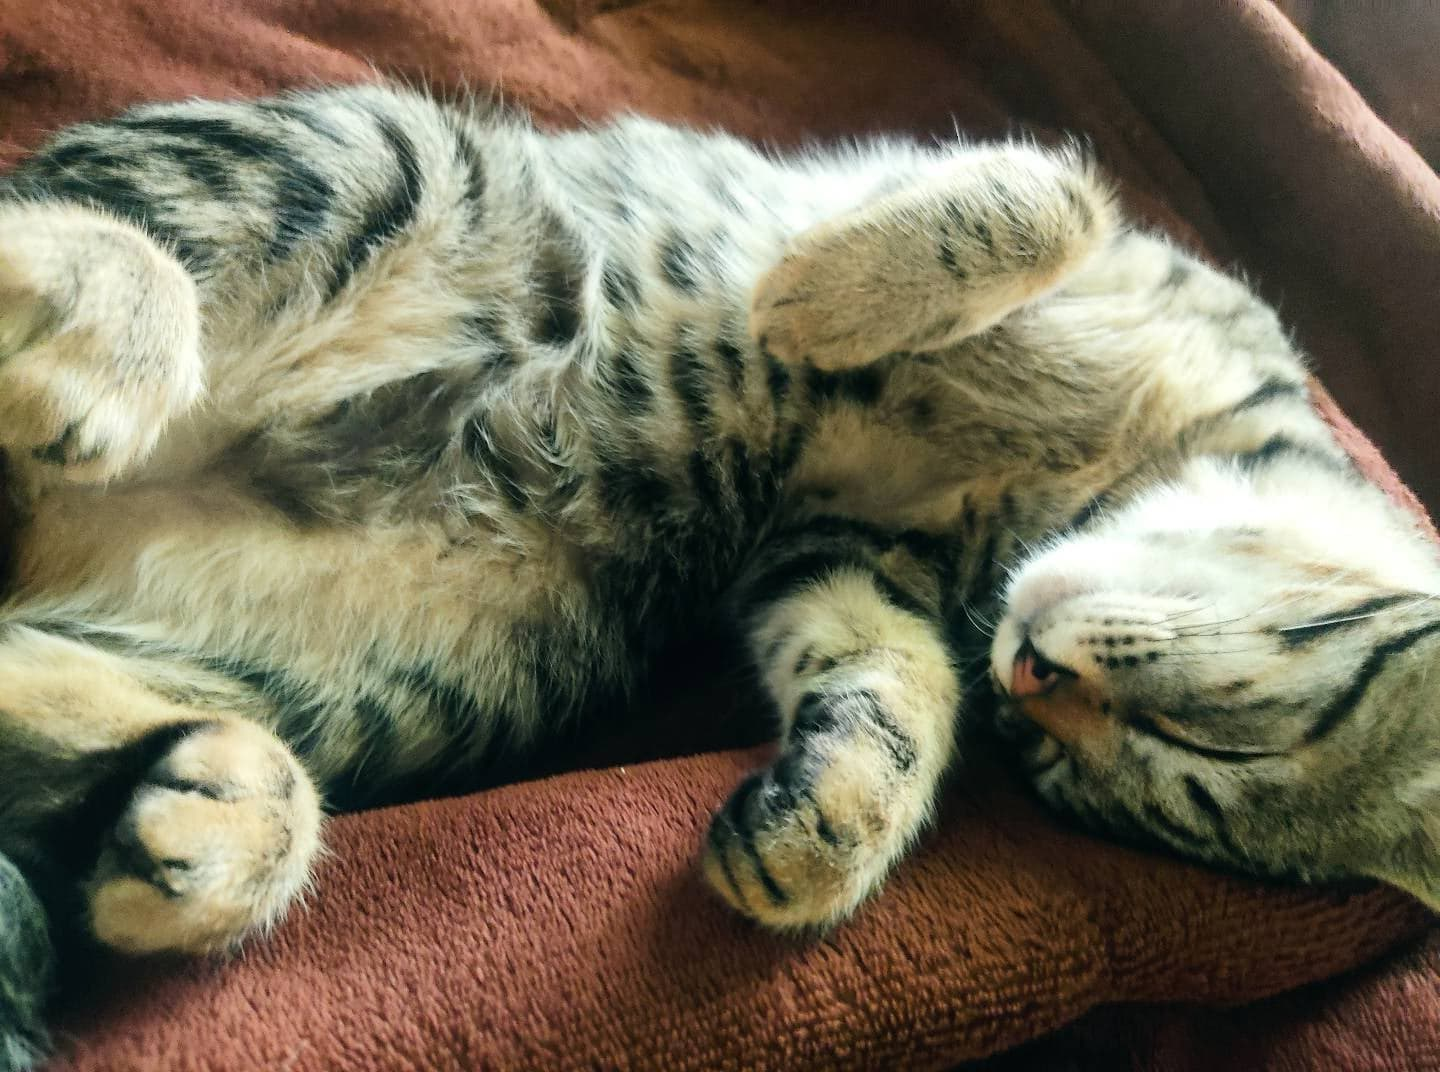
\includegraphics[width=8cm, height=6cm]{Mili.jpg}
\end{document}
